\chapter{Proposta}

	Em \cite{winikoff2014testability} um grafo de controle de fluxo foi utilizado para avaliar a testabilidade de um sistema BDI. A proposta deste trabalho é avaliar a testabilidade de um SMA utilizando o Moise como modelo de organização e empregando rede de Petri como ferramenta de descrição e análise. Partindo como base o trabalho de \cite{winikoff2017bdi} o grafo de controle de fluxo apresentado na Figura \ref{fig:control_fluxo} foi transformado em uma RP Figura \ref{fig:cf_rp}.

\begin{figure}[ht]
\centering
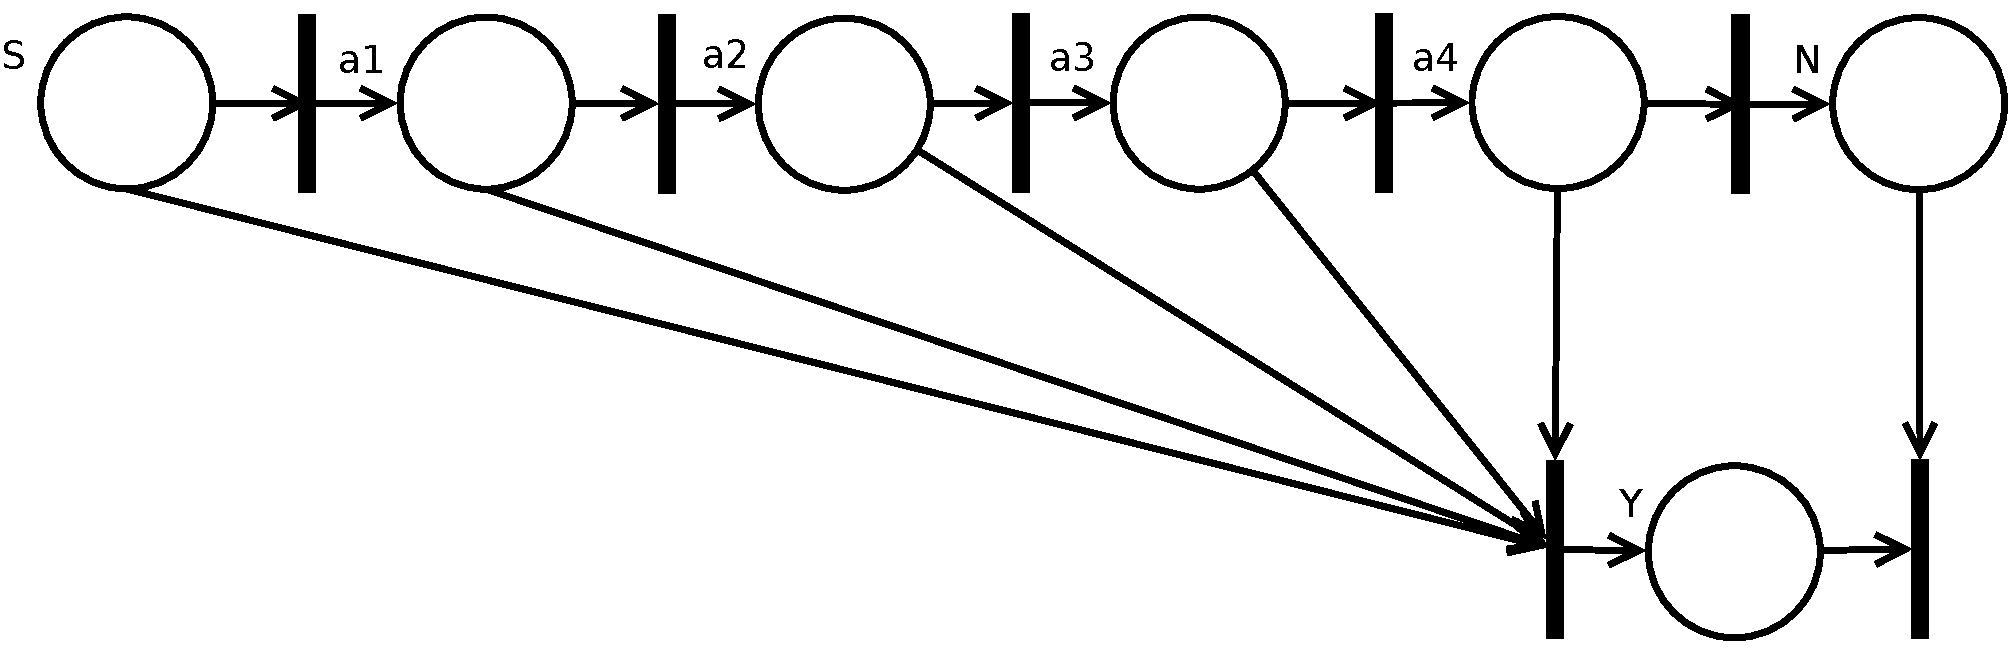
\includegraphics[scale=0.4]{imagens/cf_rp.pdf}
\caption{RP do grafo de controle de fluxo.}
\label{fig:cf_rp}
\end{figure}
    

  Para apresentar a proposta utilizando o Moise será utilizado um exemplo exposto em \cite{hubner2003modelo}. O exemplo consiste em um grupo para seleção para um curso de pós-graduação de uma instituição de ensino, a Figura \ref{fig:ee_exemplo} representa a especificação estrutural.
  
\begin{figure}[ht]
\centering
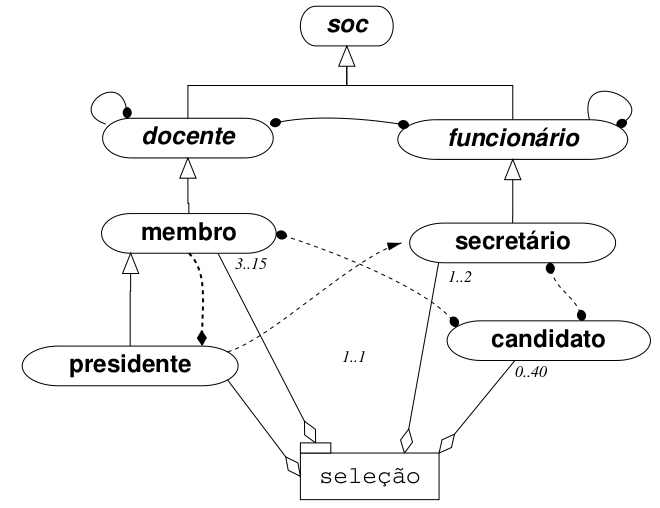
\includegraphics[scale=0.4]{imagens/modelo2.png}
\caption{Especificação Estrutural proposta para o exemplo \cite{hubner2003modelo}.}
\label{fig:ee_exemplo}
\end{figure}
  
  A EF no nível individual é representado pelas missões, e no nível coletivo pelos Esquemas Sociais (ES). Um ES é essencialmente uma árvore de decomposição de metas globais. Um ES para o exemplo proposto é representando na Figura \ref{fig:es_exemplo}.
  
\begin{figure}[ht]
\centering
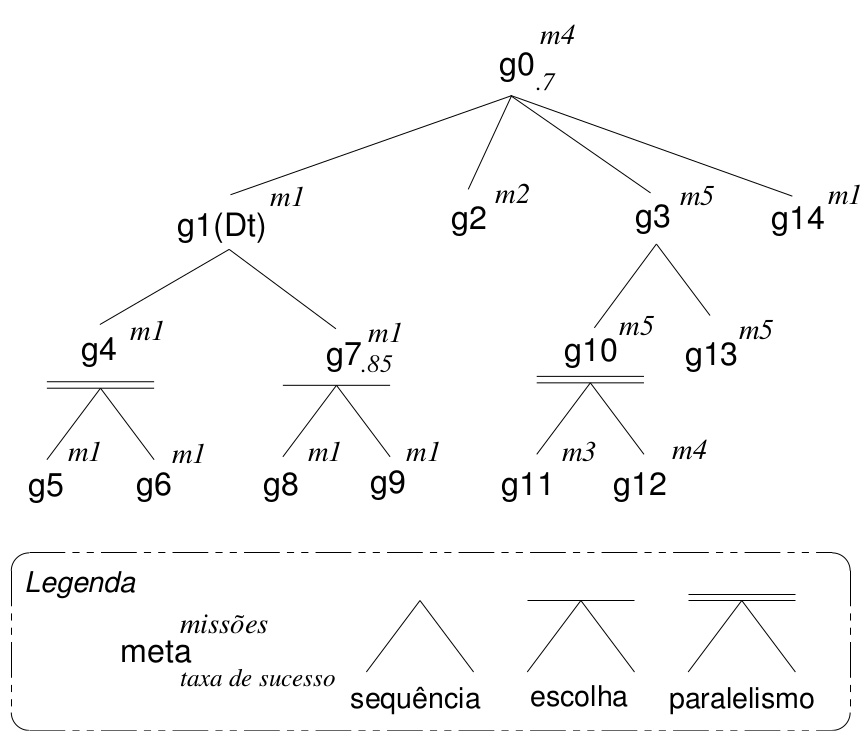
\includegraphics[scale=0.35]{imagens/ES2.png}
\caption{Esquema Social para o exemplo \cite{hubner2003modelo}.}
\label{fig:es_exemplo}
\end{figure}

Os diferentes papéis do exemplo possuem diferentes missões, um agente no papel de candidato, tem a missão $m1$. Para cumprir esta missão o candidato deve ter como objetivo as metas ($g1, g4, g5, g6, g7, g8, g9$ e $g14$), a descrição das metas está na Tabela \ref{tab:desc_metas}.

\begin{table}[ht]
\centering
\caption{Descrição das metas do exemplo \cite{hubner2003modelo}.}
\label{tab:desc_metas}
\begin{tabular}{@{}ll@{}}
\toprule
meta   & descrição                                             \\ \midrule
g0     & o/a candidato/a é aceito no programa de pós-graduação \\
g1(Dt) & a documentação é recebida no prazo                    \\
g2     & a documentação está correta                           \\
g3     & o/a candidato é aprovado pela comissão                \\
g5     & o/a candidato/a tem toda a documentação necessária    \\
g6     & o/a candidato/a tem um/a orientador/a                 \\
g7     & a inscrição está submetida                            \\
g8     & submissão eletrônica                                  \\
g9     & submissão por correio                                 \\
g11    & uma reunião está marcada                              \\
g12    & um relator está indicado                              \\
g13    & o projeto do candidato é avaliado                     \\
g14    & o formulário de matrícula preenchido é recebido      \\ \bottomrule
\end{tabular}
\end{table}


Assim através da árvore de metas globais é transformada em uma RP de acordo para cada missão Figura \ref{fig:missoes_rp}.


\begin{figure}[ht]
\centering
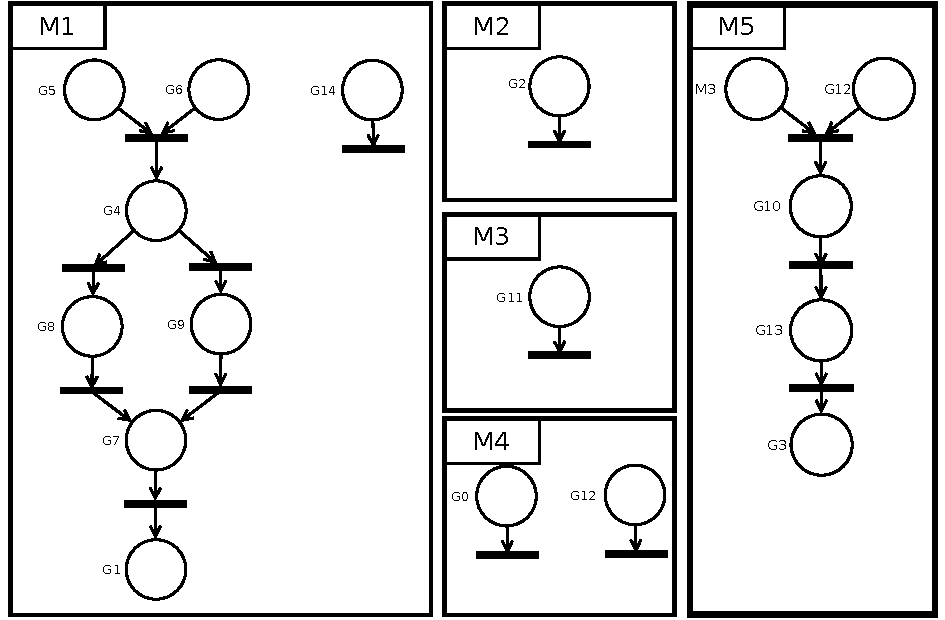
\includegraphics[scale=1]{imagens/RPGoals.pdf}
\caption{Transformação das missões do exemplo em RP.}
\label{fig:missoes_rp}
\end{figure}


\section{Cronograma}

\begin{table}[ht]
\centering
\caption{Cronograma de atividades}
\label{my-label}
\begin{tabular}{|l|c|c|c|c|c|c|}
\hline
\multicolumn{7}{|c|}{Cronograma}                                                                                                                                                                                  \\ \hline
                                                & \multicolumn{1}{l|}{Nov} & \multicolumn{1}{l|}{Dez} & \multicolumn{1}{l|}{Jan} & \multicolumn{1}{l|}{Fev} & \multicolumn{1}{l|}{Mar} & \multicolumn{1}{l|}{Abr} \\ \hline
Qualificação                                    & x                        &                          &                          &                          &                          &                          \\ \hline
Escrita de Artigo                               & x                        & x                        &                          &                          &                          &                          \\ \hline
Desenvolvimento da Metodologia para testes      & x                        & x                        & x                        &                          &                          &                          \\ \hline
Desenvolvimento de Estudos de Caso              &                          &                          & x                        & x                        & x                        &                          \\ \hline
Análise dos Resultados                          &                          &                          &                          &                          & x                        & x                        \\ \hline
Escrita Dissertação                             & x                        & x                        & x                        & x                        & x                        & x                        \\ \hline
Escrita de um Artigo com Resultados da Pesquisa &                          &                          &                          &                          & x                        & x                        \\ \hline
Defesa Mestrado                                 &                          &                          &                          &                          &                          &                          \\ \hline
\end{tabular}
\end{table}